\documentclass{report}

\usepackage[utf8]{inputenc}
\usepackage{graphicx}
\usepackage{wrapfig}
\usepackage{subfig}

\begin{document}

\title{Flappy Penguin - Projekttagebuch}
\author{Stefan Cimander}
\date{}

\maketitle


\section*{20. Juni 2016}

\subsubsection*{Projektbeginn}

Ein Teil der HCI-Vorlesung wurde von unserer Gruppe dazu genutzt, Ideen für das Abschlussprojekt zu generieren und daraus ein konkretes Konzept zu erarbeiten. Folgende Einschränkungen wurden dabei vorgegeben:

\begin{itemize}
	\item Im Rahmen des Projekts soll ein Spiel entwickelt werden
  	\item Dabei soll der Herzschlags- oder Atemsensor verwendet werden
  	\item Ein Alltagsgegenstand (z.B. Kuscheltier) soll als Steuergerät dienen.
  	\item Das System soll den Q-Learning-Algorithmus integrieren
\end{itemize}

\noindent Wir diskutieren über Möglichkeiten, bekannte Spieleklassiker anzupassen, oder ein eigenes Spielkonzept zu entwerfen. Im Gespräch waren ein vom Puls abhängiges \textit{Tetris}, ein Jump-And-Run Spiel wie \textit{Thomas was alone} sowie die Veränderung von \textit{Breakout}. Unter anderem diskutierten wir allerdings auch darüber, \textit{Flappy Bird} auf irgendeine Weise zu erweitern.


\subsubsection*{Projektidee}

Über den Gedanken, den Spieler in ein Unterwasserszenario zu versetzen, in welchem er sein Ziel nur erreicht, wenn er regelmäßig ein wenig die Luft anhält, entstand die Idee von Flappy Penguin:

\begin{itemize}
	\item Der Spieler spielt einen Pinguin, der unter der Wasseroberfläche verschiedenen Hindernissen wie zum Beispiel Eisschollen ausweichen muss. Analog zum bekannten Spiel \textit{Flappy Bird} kann der Pinguin lediglich nach oben gesteuert werden und sinkt anschließend von alleine wieder ab. Hinzu kommt, dass dem Spieler nur eine begrenzte Anzahl an \textbf{Luftblasen} zur verfügung steht um mit dem Pinguin unter Wasser zu tauchen. Sind die Luftblasen verbraucht, muss der Pinguin, damit das Spiel nicht verloren geht, an die Wasseroberfläche tauchen und neue Luftblasen einatmen.
	\item Die Idee der Integration eines \textbf{Atemsensors} ist, dass bei jedem Einatmen des Spielers eine Luftblase verbraucht wird, falls sich der Kopf des Pinguins unterhalb der Wasseroberfläche befindet. Ist der Kopf oberhalb der Wasseroberfläche, kann der Spieler durch Einatmen eine Luftblase zurückbekommen.  
	\item Um die Steuerung intuitiver zu gestalten, wird ein \textbf{Pinguin-Kuscheltier} mit einem Drucksensor versehen. Drückt der Spieler das Kuscheltier gibt der Sensor das Signal zum Auftauchen
	\item Eine endgültige Idee für die Einbeziehung des Q-Learning-Algorithmus steht zu diesem Zeitpunkt noch nicht fest, in der Diskussion stehen das Platzieren von zusätzlichen Luftblasen, die der Spieler einsammeln kann, oder das Einfügen eines vom Computer gesteuerten Pinguins. 
\end{itemize}


\subsubsection*{Aufgabenverteilung}

Nachdem wir uns auf ein grobes Konzept für unsere Projektidee geeinigt haben, diskutieren wir das weitere Vorgehen. Gernot bietet an, sich um den Brustgurt mit dem Atemsensor zu kümmern, Thomas schlägt das Framework \textit{create.js} für die Entwicklung der Spieloberfläche vor, woraufhin wir beschließen, dass Thomas und Martin sich in das Framework einarbeiten und ich mich mit der Projektorganisation und der Dokumentation unserer Projektidee befasse, sowie einen kurzen Projektplan erstelle.


\section*{23. Juni 2016}

\subsubsection*{Spiel-Prototyp}

Zwischen zwei Vorlesungen präsentiert Thomas der Gruppe einen ersten frühen Prototyp der graphischen Oberfläche des Spiels. Auch Springen und Erkennen von Kollisionen mit Eisblöcken sind bereits implementiert, was es uns ermöglicht, erste Spielversuche zu starten. Das Design des Pinguins und die Animation der Umgebung kommt bei der Gruppe sehr gut an. Wir entscheiden, dass diese Projektidee in dem festgelegten Zeitraum umsetzbar ist und dass es deswegen nicht notwendig ist, die Idee zu überarbeiten. \\

\noindent Ein Ausschnitt des Prototyps der graphischen Oberfläche ist in Abbildung \ref{fig:prototype} zu sehen. Für die Pinguin-Spielfigur existiert auch eine weibliche Variante.

\begin{figure*}
	\center
	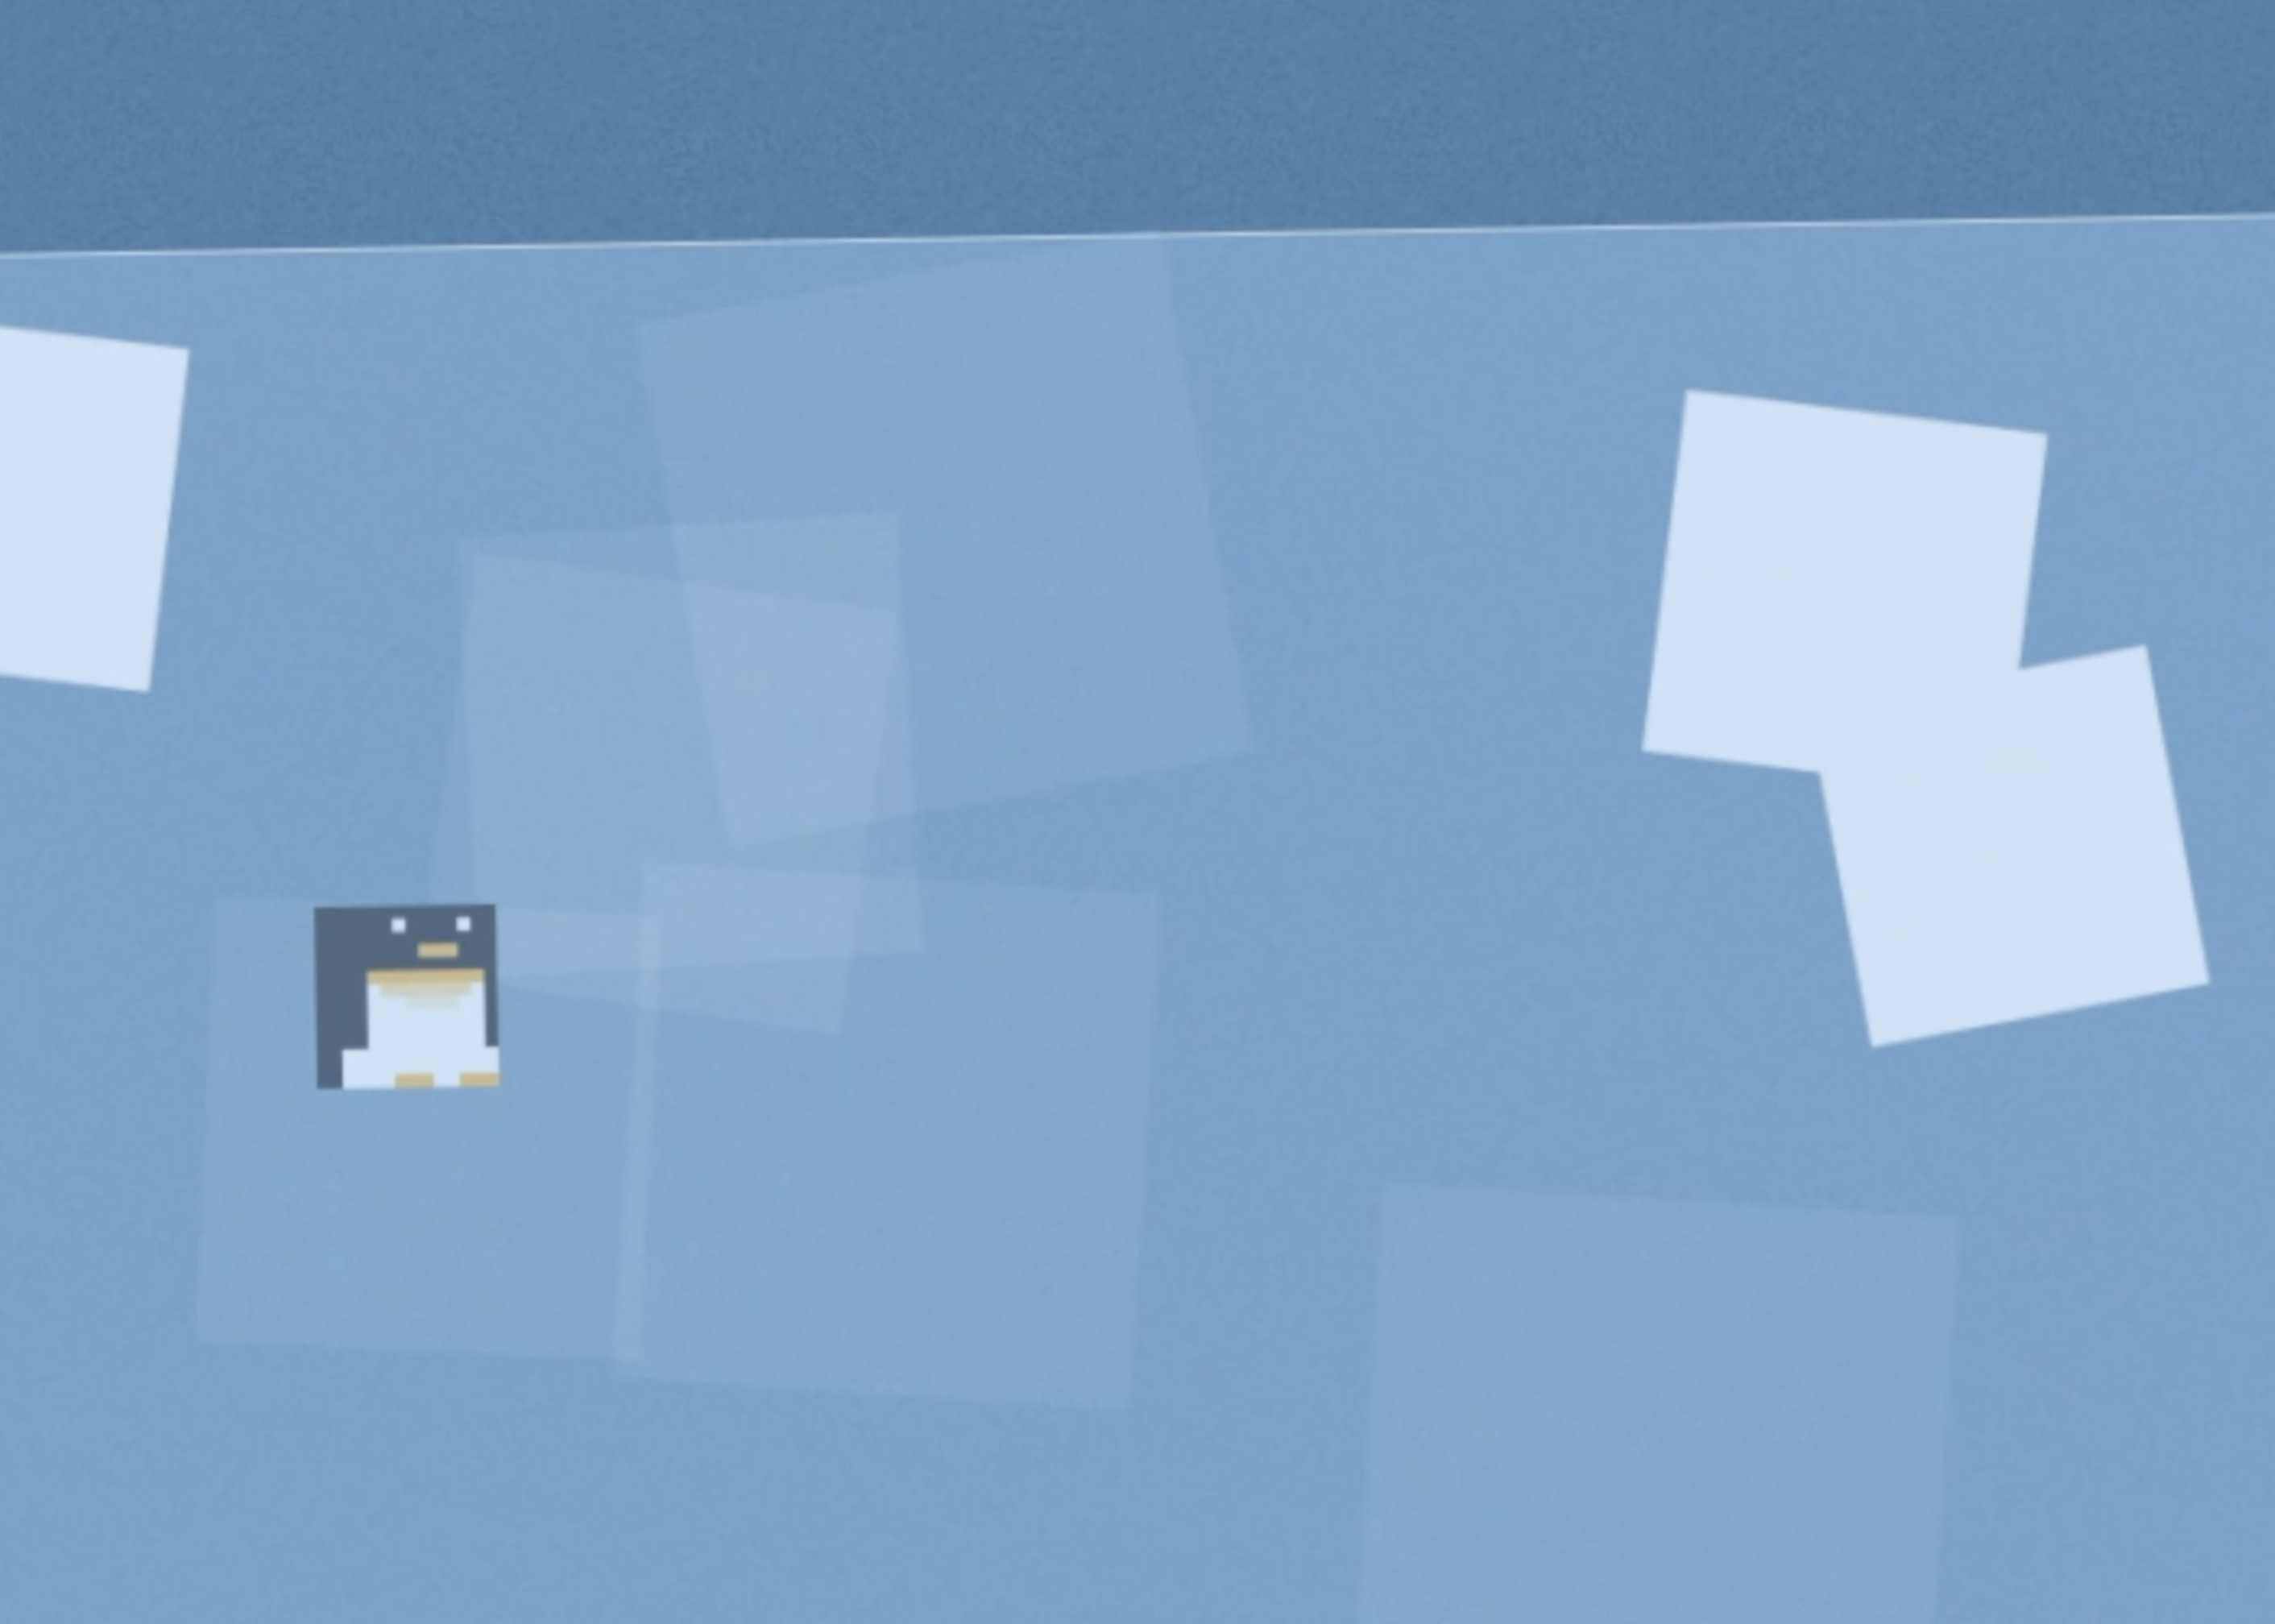
\includegraphics[width=100mm]{img/prototype}
	\caption{Prototyp der graphischen Spieloberfläche}
	\label{fig:prototype}
\end{figure*}
\pagebreak


\section*{25. Juni 2016}

\subsubsection*{Dokumentation und Projektplan}

Zu Hause formuliere ich unserer Projektidee und fasse die wesentlichen Eigenschaften des zu entwickelnden Spiels zusammen. Außerdem stelle ich einen Projektplan auf, der die folgenden drei Abschnitte enthält:

\begin{description}
	\item [Aufgabenverteilung] dokumentiert die Verantwortlichkeiten der Teammitglieder,
	\item [Projektmeilensteine] definieren feste Zeitpunkte zur Fortschrittskontrolle,
	\item [Risiken] erläutern und bewerten potenzielle Gefährdungen für das Projekt.
\end{description}

\noindent Da zum jetzigen Zeitpunkt noch nicht für jede Projektanforderung eine Umsetzung in unser Spiel gefunden ist, werden die Dokumentation und der Projektplan während dem weiteren Projektverlauf durchgehend angepasst. So ist beispielsweise noch die endgültige Entscheidung zu treffen, wie der Q-Learning-Algorithmus in das Spiel integriert werden soll. Auch sind  die weiteren Verantwortlichkeiten der Teammitglieder noch nicht endgültig festgelegt.


\section*{27. Juni 2016}

\subsubsection*{Abstimmung des Projektplans}

Zu Beginn unseres Treffens im Rahmen der Vorlesung stimme ich den von mir erstellten Projektplan mit der Gruppe ab. Wir beschließen, uns spätestens auf eine Möglichkeit festzulegen, den Q-Learning-Algorithmus in unser Spiel zu integrieren. Außerdem wollen wir an der bisherigen Rollenverteilung festhalten und uns falls nötig in unseren Aufgaben gegenseitig unterstützen.


\subsubsection*{Demonstration des Atemsensors}

Des Weiteren präsentiert uns Gernot den Atemsensor, den er auf einem Brustgurt befestigt hat. Die anschließende Integration über den Arduino und Node.js in das Spiel sieht nach einer ersten Testphase sehr vielversprechend aus. 


\subsubsection*{Dokumentation der technischen Umsetzung}

Den Rest der Vorlesung nutze ich zur Dokumentation der von uns verwendeten Technologien und Frameworks. Dazu gehören ein \textit{Arduino} Mikrokontroller, ein \textit{Node.js} Webserver, das \textit{Create.js} Games Framework sowie ein Dehnungssensor zur Atmungserkennung und ein Biegesensor zur Steuerung mit dem Kuscheltier. \\

\noindent Abbildung \ref{fig:documentation} zeigt eine Übersicht der fertigen Dokumentation, einschließlich des Titelblatts, der Beschreibung der Projektidee und technischen Umsetzung, sowie des Projektplans.

\begin{figure*}
	\center
	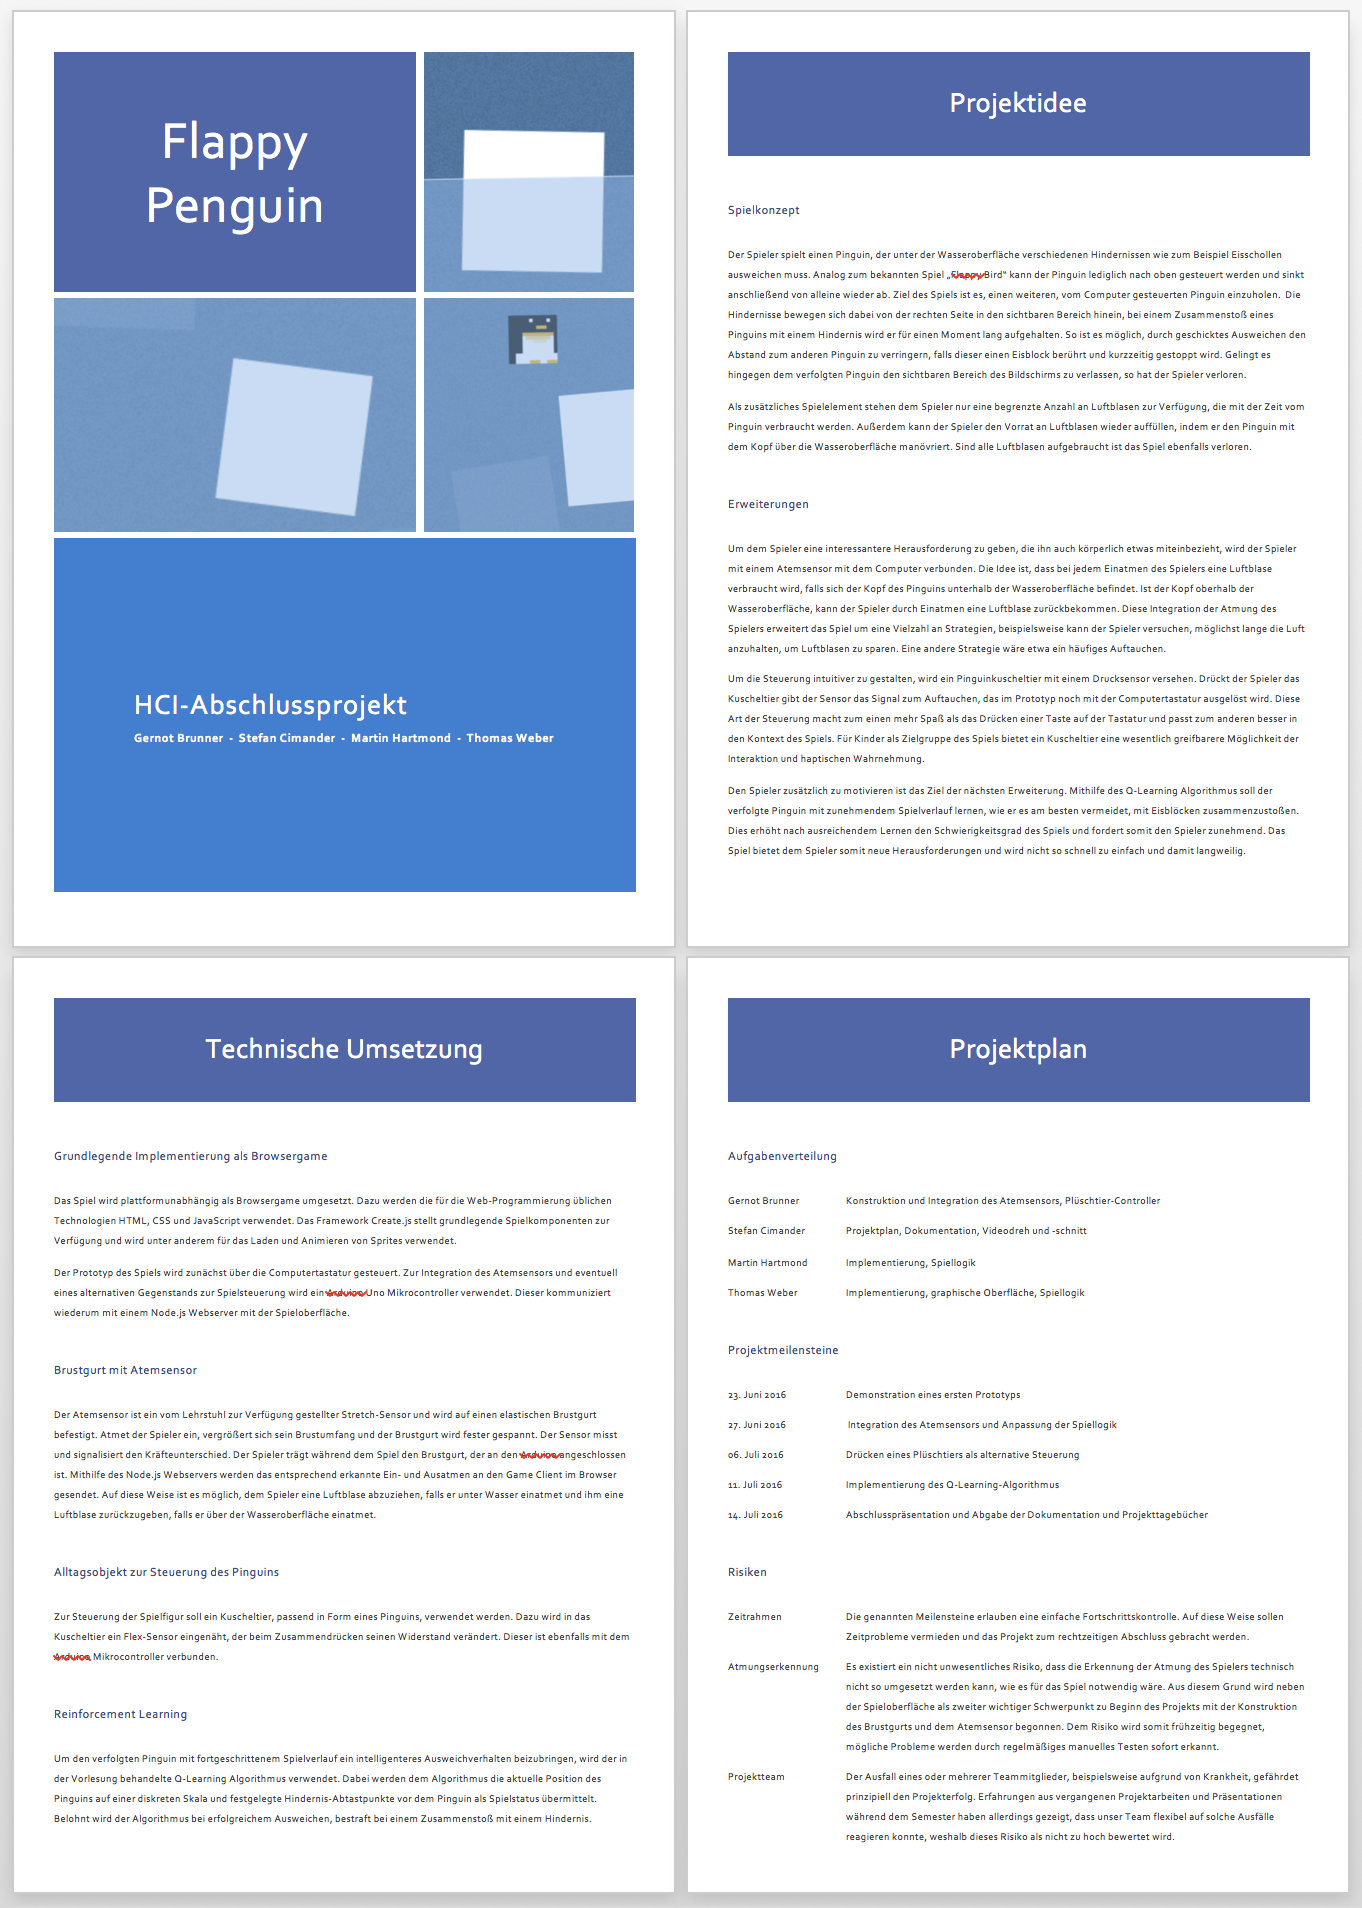
\includegraphics[width=130mm]{img/documentation}
	\caption{Übersicht unserer Projektdokumentation}
	\label{fig:documentation}
\end{figure*}
\pagebreak



\section*{4. Juli 2016}

\subsubsection*{Präsentationsfolien}

Das heutige Treffen nutzte ich zur Erstellung erster Präsentationsfolien. Zwar sind es noch zehn Tage bis zur Präsentation, dennoch möchte ich rechtzeitig damit beginnen, um genug Zeit für nachträgliche Änderungen und die Erstellung unseres Videos übrig zu haben. Das gekachelte Design der Folien orientiert sich an der Graphik des Spiels und ist, genau wie die Projektdokumentation farblich an das eisige Unterwasserszenario angelehnt. Nach Absprache des Folien-Layouts mit dem Team erstelle ich die Vorlagen für verschiedene Abschnitte der Präsentation. Die Titelfolie der Präsentation ist in Abbildung \ref{fig:presentation} zu sehen.


\subsubsection*{Drehbuch für Projektvideo}

Gemeinsam mit Gernot mache ich mir anschließend Gedanken über das zu erstellende Projektvideo. Wir erstellen ein erstes Drehbuch, das die folgenden wichtigsten Kategorien von Szenen umfasst:

\begin{itemize}
	\item Demonstration der Hardware (Brustgurt \& Pinguin-Kuscheltier)
	\item Bildschirmaufnahmen des Spiels zum Erklären des Spielkonzepts
	\item Aufnahme des Spielers und seinen (Re-)Aktionen während dem Spielen
\end{itemize} 

\noindent Ich biete an, mich um die Aufnahme der Videos sowie um die Bearbeitung und Schnitt zu kümmern.

\begin{figure*}
	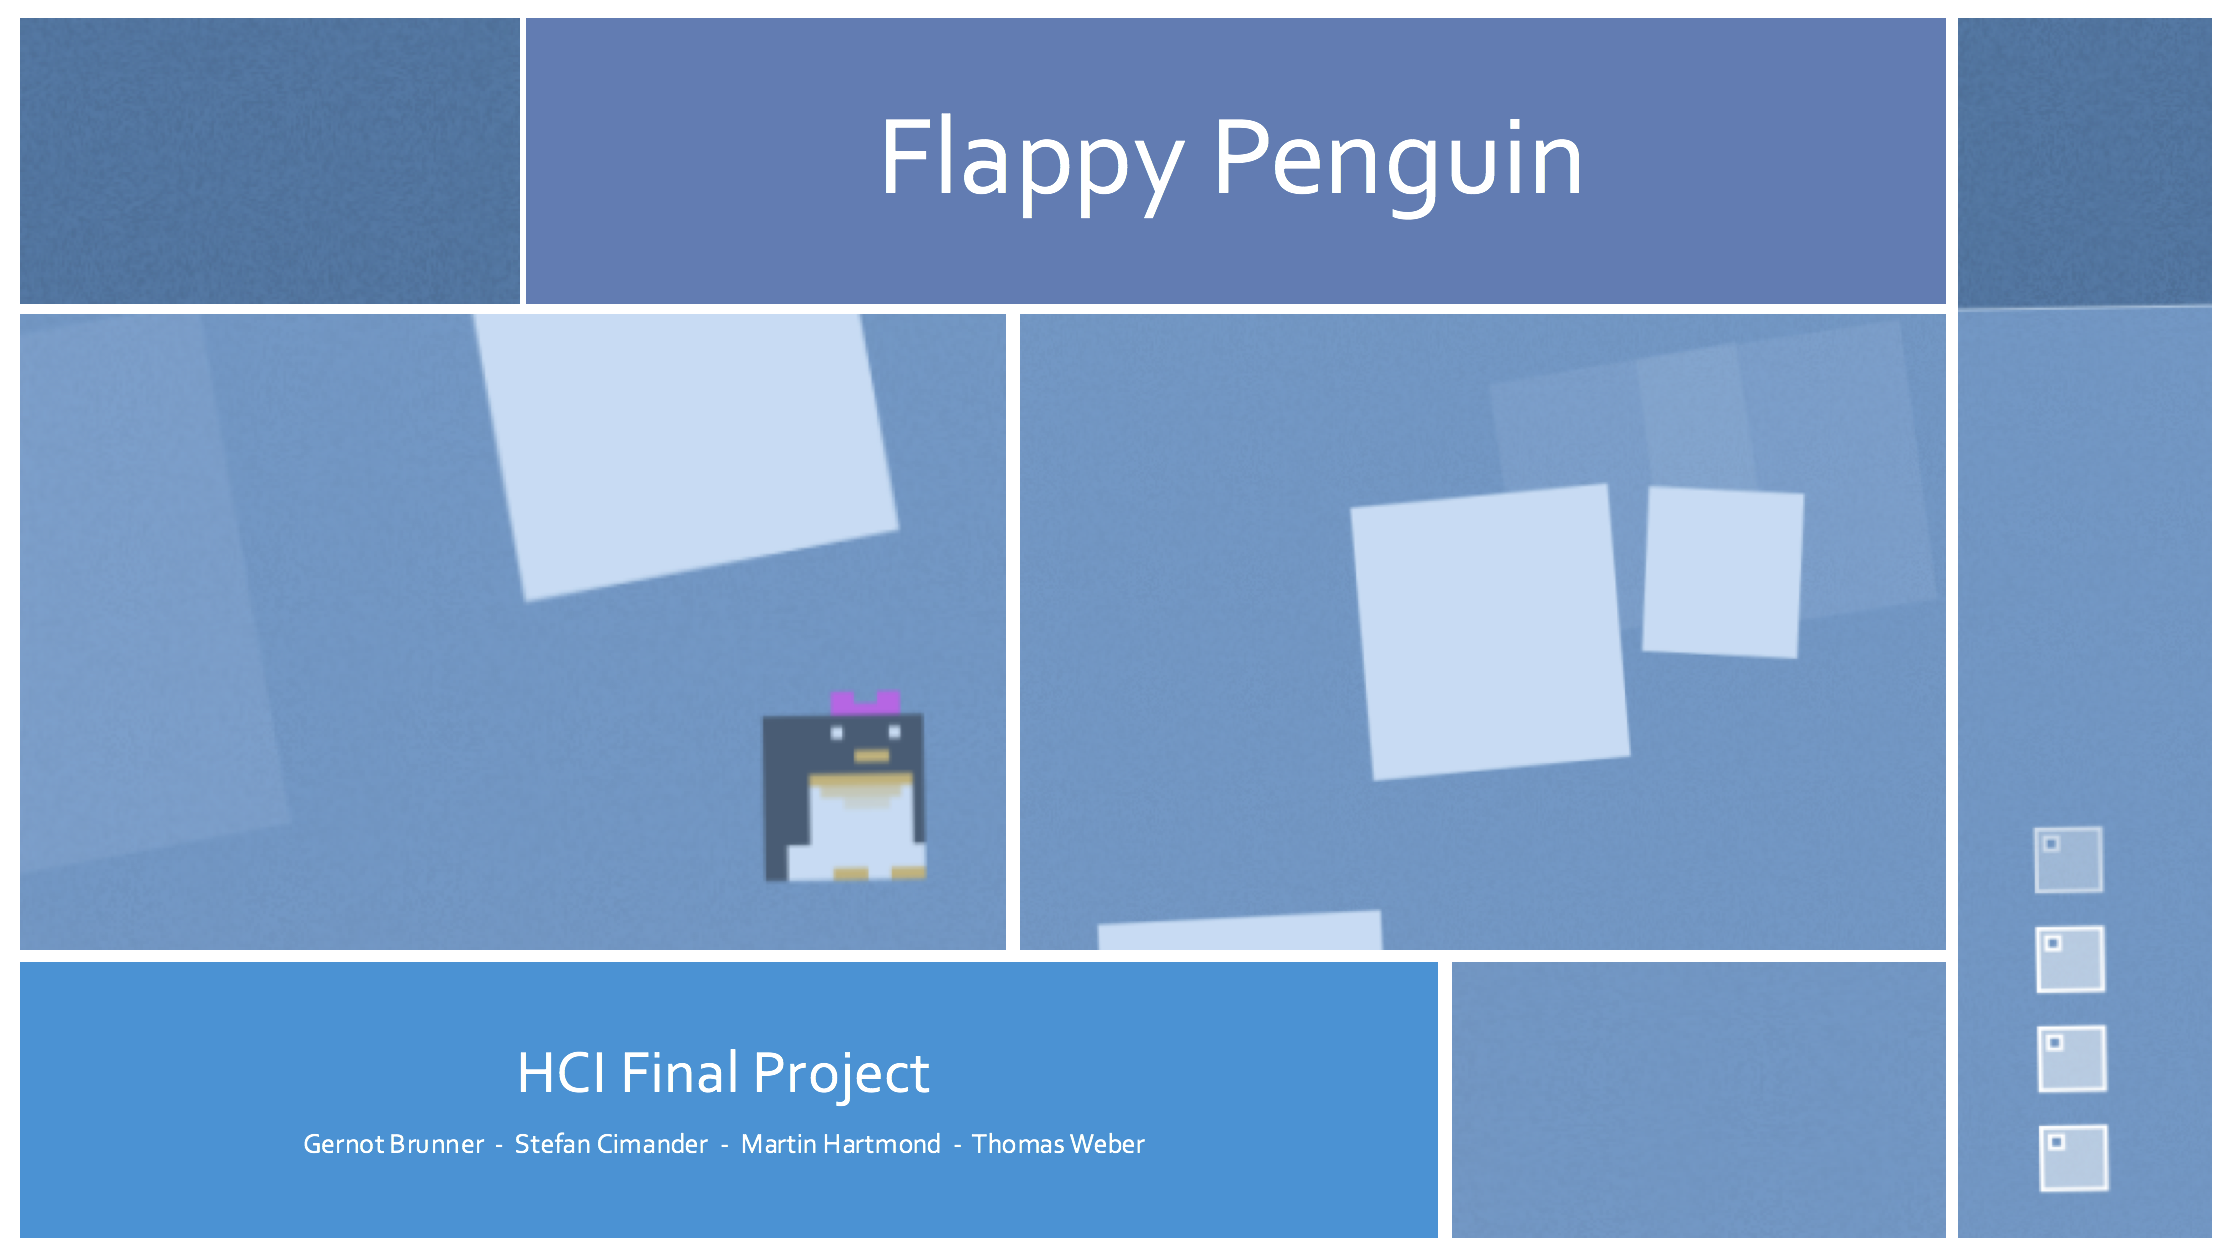
\includegraphics[width=120mm]{img/presentation}
	\caption{Titelfolie unserer Präsentation}
	\label{fig:presentation}
\end{figure*}
\pagebreak



\section*{9. Juli 2016}

\subsubsection*{Vorbereitungen für Videoaufnahmen}

Als Vorbereitung für das Drehen der Videos experimentiere ich zu Hause mit der Möglichkeit gleichzeitig einen Ausschnitt des Bildschirms und ein Video mit der Webcam meines Laptops aufzunehmen. Auf diese Weise ist es möglich die Aufnahmen des Spielgeschehens mit denen der Reaktionen des Spielers zu synchronisieren. Zu meiner positiven Überraschung ist das mit dem \textit{QuickTime Player} ohne Probleme möglich. \\

\noindent Außerdem mache ich mich mit dem Bearbeitungsprogramm \textit{iMovie} vertraut und suche nach einem geeigneten Template und passender Musik. Als abschließende Vorbereitung installiere ich \textit{Node.js} und die für unser Spiel notwendigen \textit{npm}-Packages. Somit ist für die Videoaufnahmen am Montag alles bereit.



\section*{11. Juli 2016}

\subsubsection*{Abschlussbesprechung}

Abschließend vor der Präsentation am Donnerstag erklärt Thomas uns außerdem, wie er den Q-Learning-Algorithmus implementiert hat. Wir haben uns letzte Woche, dafür entschieden die Variante mit dem vom Computer gesteuerten Pinguin auszuwählen. Das angepasste Ziel des Spiels ist daher den anderen Pinguin einzuholen und zu fangen. Auch ist das Spiel nicht mehr verloren, sobald ein Eisblock berührt wird, sondern der kollidierende Pinguin wird lediglich kurz abgebremst. Allerdings ist es nun möglich das Spiel zu verlieren, falls der zu fangende Pinguin aus dem für den Spieler sichtbaren Bereich entkommt. \\

Zudem ist letzte Woche der Controller in Form eines Pinguin-Kuscheltier fertig geworden. Gernot nähte dafür einen Biegesensor in das Plüschtier ein. Der Sensor wird beim Drücken des Pinguins verbogen, ändert dadurch seinen Widerstand und signalisiert diese Aktion über den \textit{Arduino} an das Spiel.


\subsubsection*{Videoaufnahmen}

Heute nehmen wir außerdem das für die Abschlusspräsentation benötigte Videomaterial auf. Gernot ist damit einverstanden, die Rolle des Spielers zu übernehmen und die Hardware zu präsentieren. Für das Drehen der Spielszenen nehmen wir wie zuvor beschrieben gleichzeitig den Bildschirm mit der graphischen Oberfläche des Spiels und den Spieler auf. Das Erklären des Brustgurts mit dem Atemsensor und des Plüschtier-Controllers nehme ich mit der Kamera eines Handys auf. \\

\noindent Abbildung \ref{fig:video} zeigt den Teil einer Videoaufnahme, bei der Gernot den Brustgurt mit dem Atemsensor vorführt und sich diesen anschließend anlegt.

\begin{figure*}
	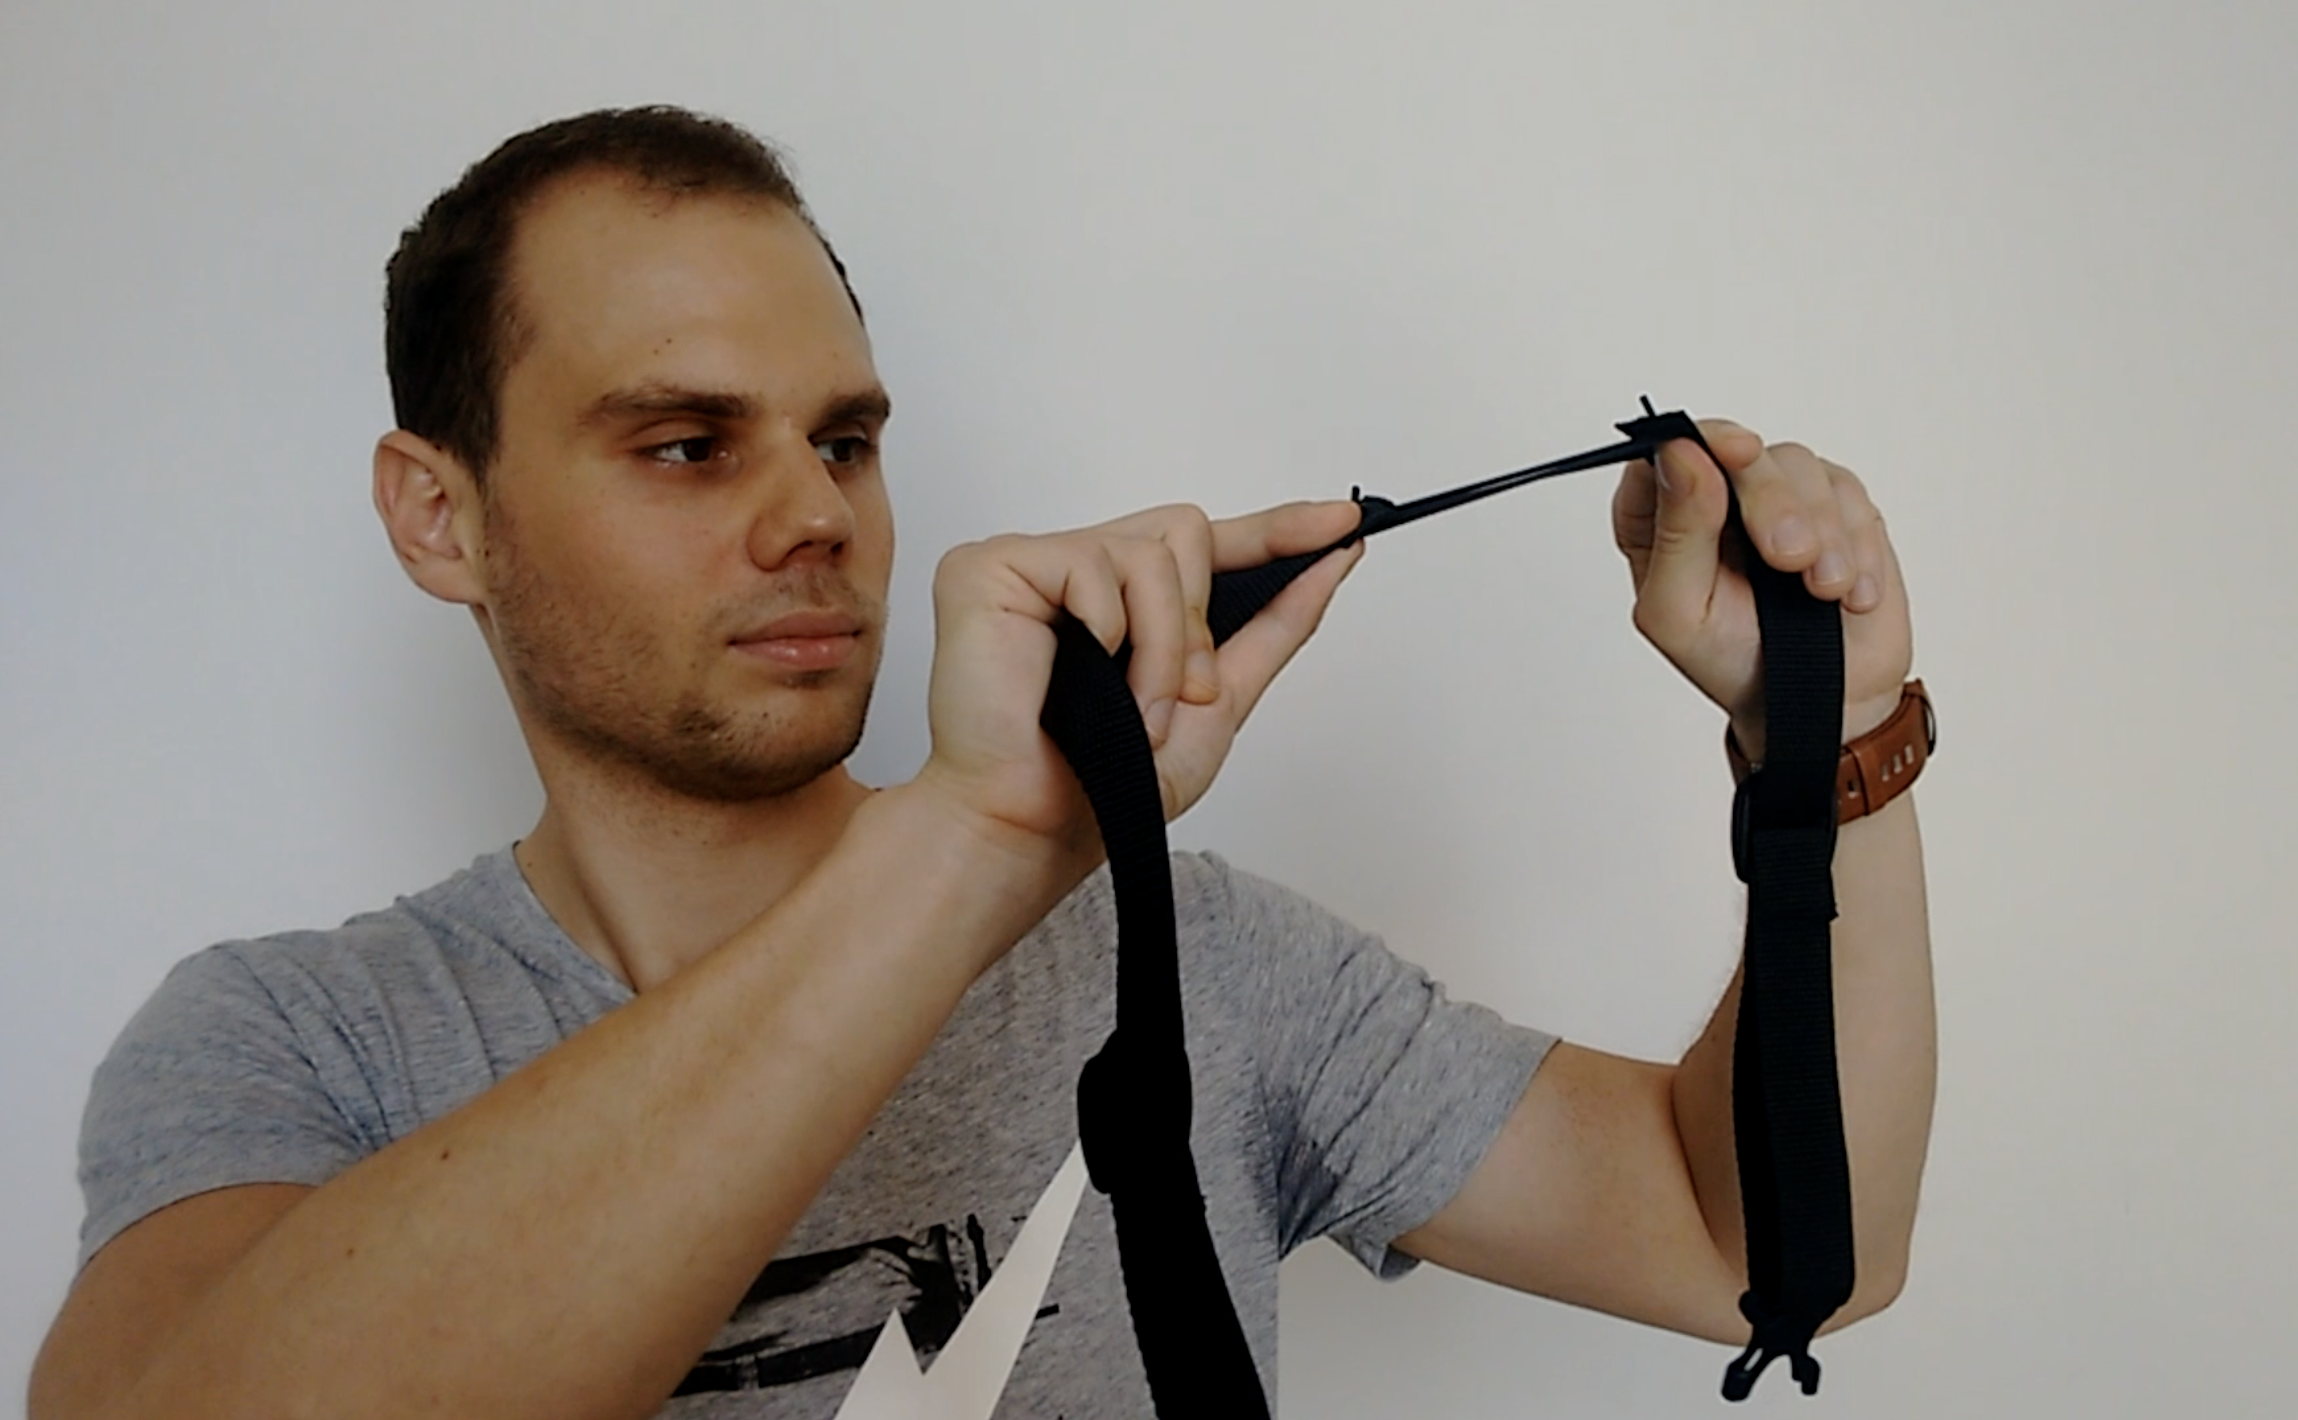
\includegraphics[width=120mm]{img/video}
	\caption{Gernot beim Vorführen des Atemsensors}
	\label{fig:video}
\end{figure*}



\section*{12. Juli 2016}

\subsubsection*{Videoschnitt}

Ich übernehme das Auswählen, Nachbearbeiten und Zuschneiden der ausgewählten Videosequenzen. Dazu orientiere ich mich an einem \textit{iMovie} Template, das für das einfache Erstellen von Filmtrailern gedacht ist. Zunächst suche ich in unserem aufgenommenen Videomaterial nach passenden Szenen, schneide diese passend zu und füge sie nacheinander in die Vorlagesequenz ein. In der nachfolgenden Abbildung ist ein Screenshot von \textit{iMovie} zu sehen, der einen Teil der fertigen Sequenz mit der grün unterlegten Audiospur zeigt. Spielszenen, die für das Video schön wären aber am Montag nicht von uns aufgenommen wurden, nehme ich nachträglich auf. Am Ende des Schneidens passe ich die Übergänge noch auf die Musik an und exportiere das fertige Video.


\subsubsection*{Probleme mit dem Controller}

Gernot teilt der Gruppe außerdem mit, dass beim Videodreh am Montag der Plüschtier-Controller kaputt gegangen ist. Im innenliegenden Biegesensor ist durch zu festes Drücken des Plüschtiers eine Lötstelle abgebrochen. Zwar versucht er noch dies zu reparieren und den Lehrstuhl um einen Ersatzsensor zu bitten, wir sollten uns allerdings eine Alternative für die zur Präsentation gehörige Demo überlegen. Ich schlage vor, auf die ursprünglich für das Springen verwendete Leertaste zurückzugreifen.

\begin{figure*}
	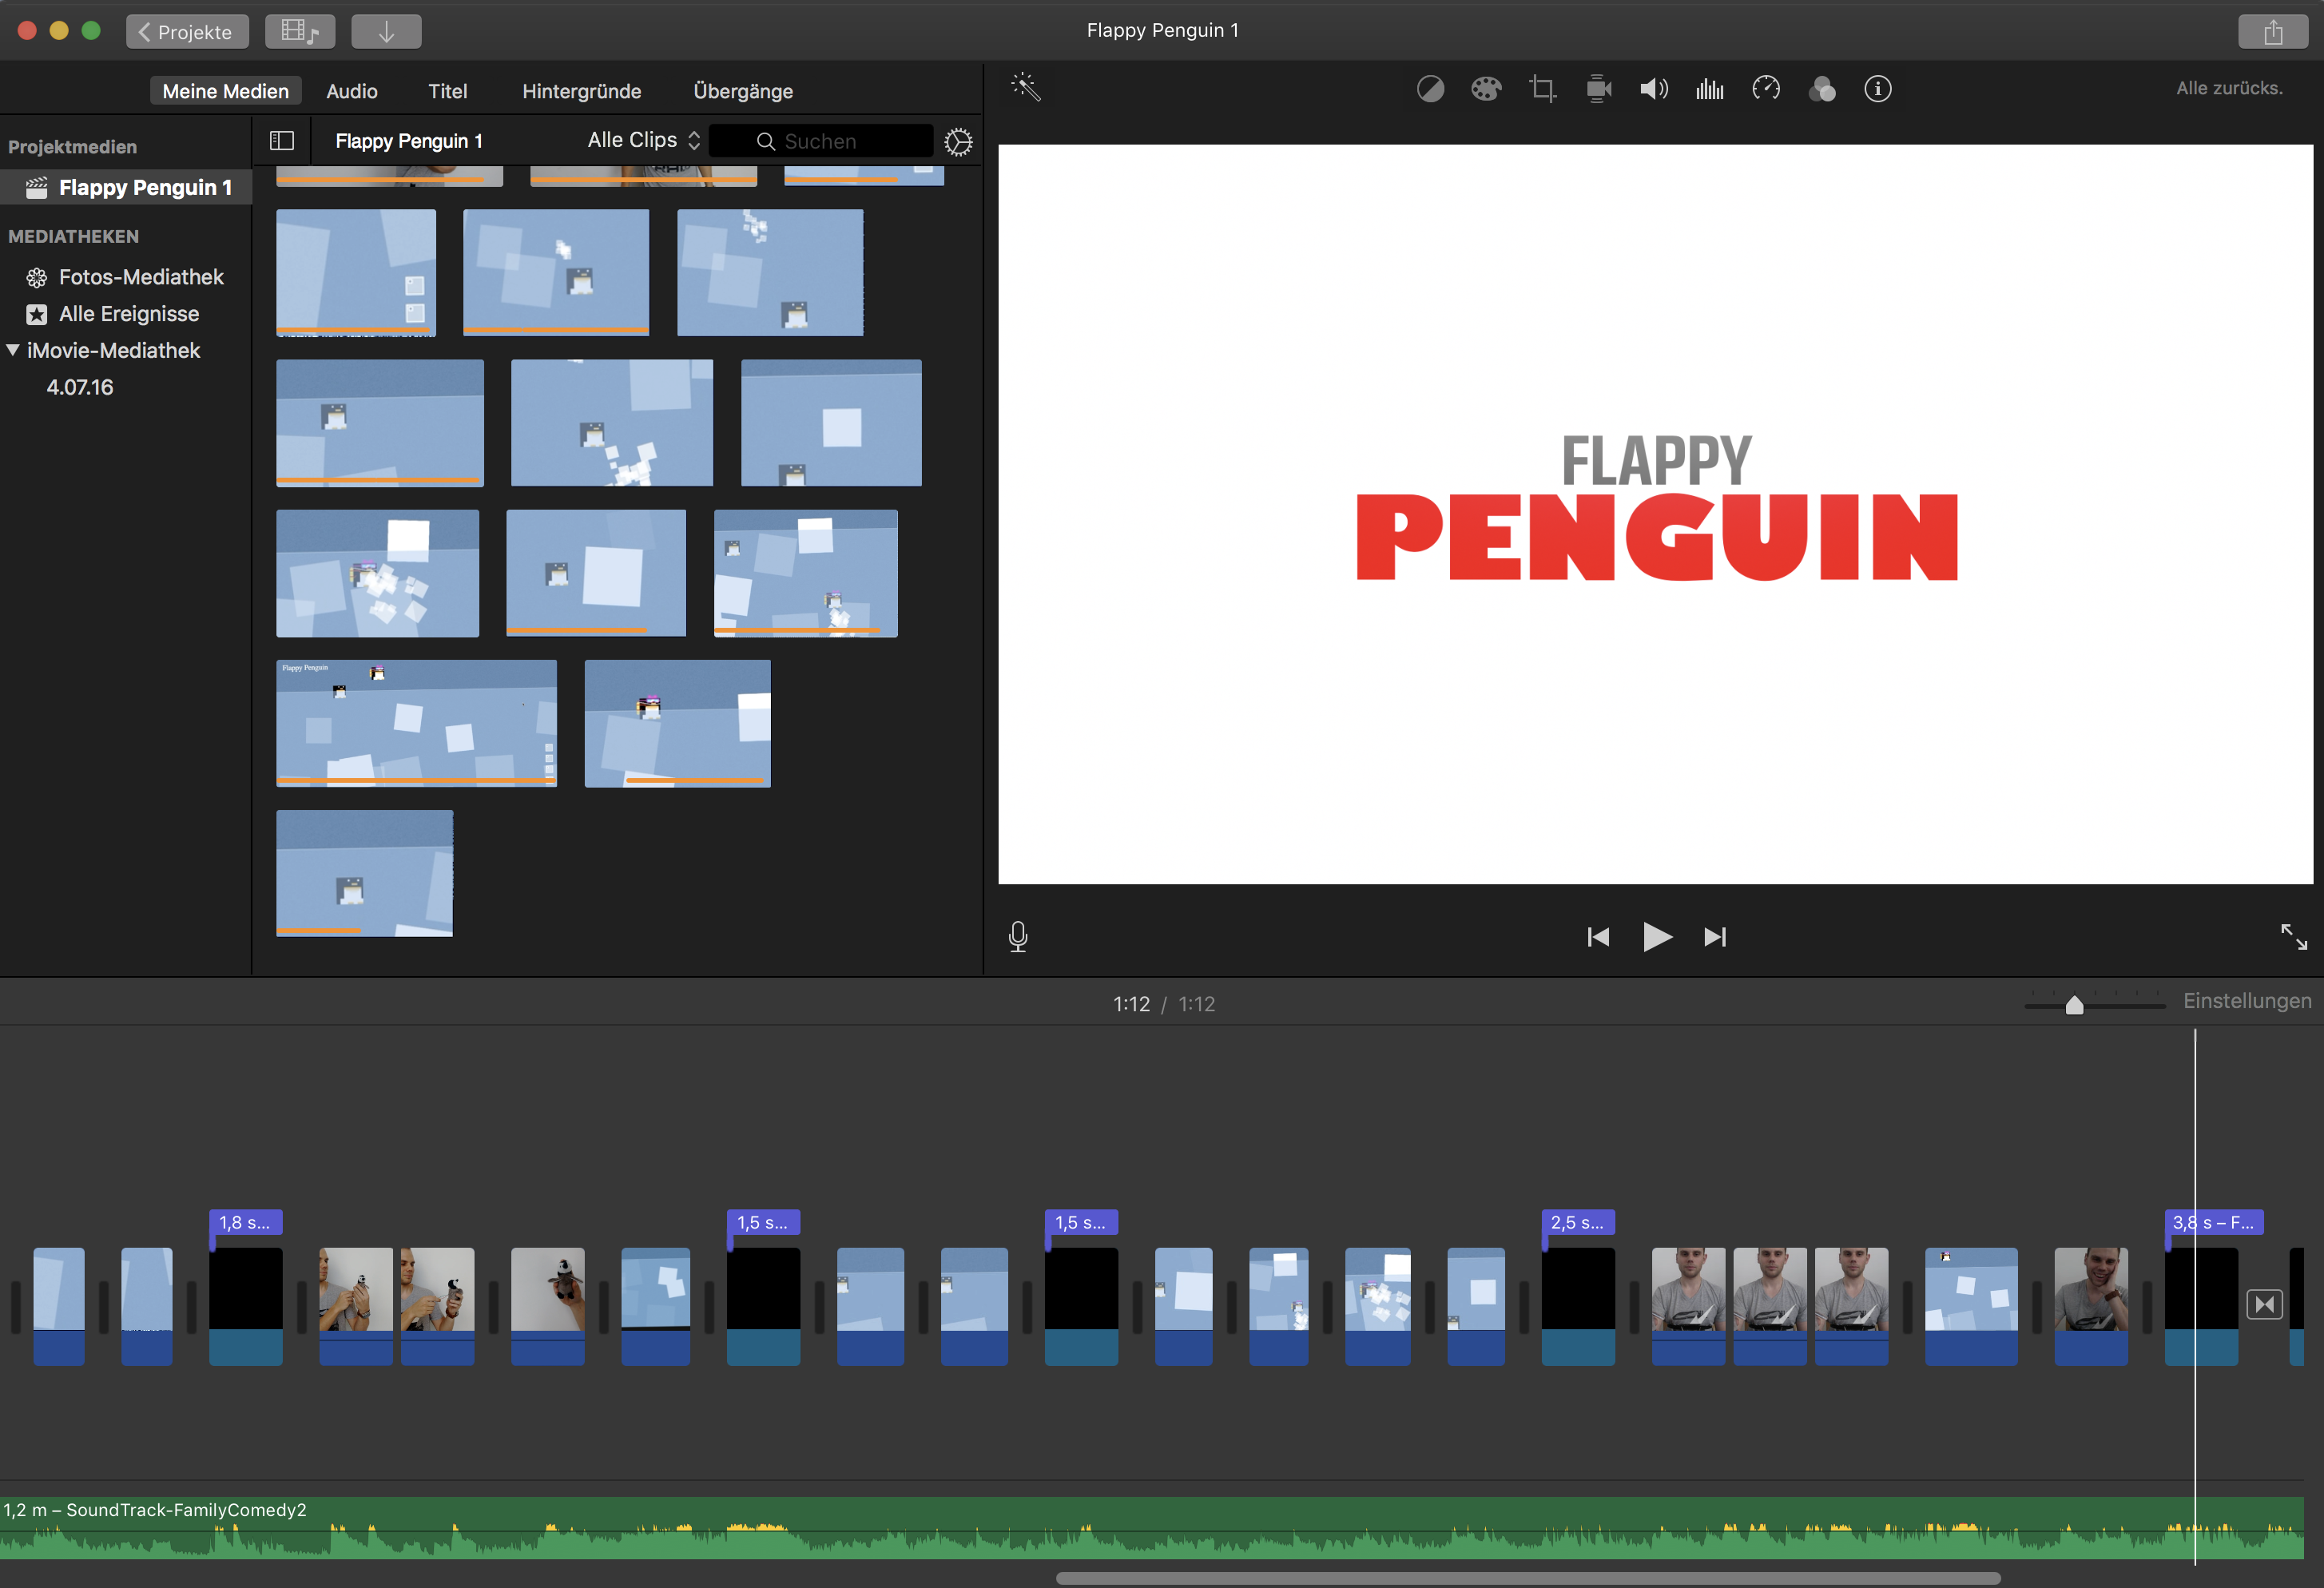
\includegraphics[width=120mm]{img/movie}
	\caption{Schneiden des Videos mit iMovie}
	\label{fig:movie}
\end{figure*}



\section*{14. Juli 2016}

\subsubsection{Controller Hotfix}

Um dem Problem des defekten Plüschtier-Controllers zu begegnen, entscheiden wir, den Presenter als Ersatz zu verwenden. Thomas passt dazu kurzfristig den Programmcode an. Auf diese Weise ist es möglich, eine vergleichbarere Spiel-\linebreak steuerung zu vermitteln, als es die Verwendung der Leertaste zulassen würde.


\subsubsection{Abschlusspräsentation}

Das Ziel ist erreicht, heute ist die Abschlusspräsentation unserer Projekte am Lehrstuhl in Augsburg. Leider vergesse ich beim Erklären des Spielprinzips näher auf die Bedeutung des Atemsensors einzugehen, weswegen die Demo etwas chaotisch abläuft. Dies liegt allerdings auch daran, dass der kurzfristige Ersatz unseres Controllers durch den Presenter nicht ganz zu Ende gedacht war. Die Tastenbelegung auf dem Presenter ist nämlich so angeordnet, dass die Taste zum Springen genau links neben einer Taste liegt, die zum Neuladen der Seite im Browser führt. Dies führt bei der Demo dazu, dass das versehentliche Drücken der falschen Taste das Spiel unterbricht und neu startet. \\

\noindent Ansonsten verläuft die Präsentation aber ungefähr so, wie wir sie uns vorgestellt haben. Rückblickend auf das Projekt können wir meiner Meinung nach sehr zufrieden mit unserer Leistung sein.

\end{document}
